\chapter{Theory and Methods}

\section{Ballistic transport \label{sec:transport} }

The Green function $G$ of a Hamiltonian $H$ is the operator that satisfies the homogenous equation 
\begin{equation}
    \left(i\hbar\frac{\partial}{\partial t}-H\right)G\left(t-t'\right)=\delta(t-t').
\end{equation}

This type of differential equations are solved taking the Fourier transform 
\begin{equation}
    \Green{H}=\int_{-\infty}^{\infty}G(t-t')e^{i\omega(t-t')/\hbar}\delta(t-t')
\end{equation}

In this new space the solution of the equation is 
$$(\omega+is -H)\Green{\omega}=I.$$ 

The term $+is$ in the previous hamiltonian is part of a mathematical trick quite common in this theory. During the whole procedure, the Green function acts on the complex field. But when we need to obtain a physical interpretation we will take the limit $s\rightarrow0$ to obtain the result for real energies. 
The next step is to decompose $\Green{H}$ in the eigenbase of the Hamiltonian $\{\ket{\alpha}\}$  by 


\begin{equation}
    \Green{\alpha,\alpha'}=\langle \alpha  \vert \Green{H}\ket{\alpha'}=\frac{\delta_{\alpha\alpha'}}{\omega - is -\ep_\alpha}=\frac{\delta_{\alpha\alpha'}(\omega + is -\ep_\alpha)}{(\omega-\epsilon_{\alpha})^{2}+s^{2}}.
\end{equation}

From the famous formula 
\begin{equation}
\lim_{s\rightarrow0}\frac{s}{(\omega-\epsilon_{\alpha})^{2}+s^{2}}=\pi\delta(\omega-\epsilon_{\alpha})
\end{equation}
we obtain 
\begin{equation}
    Im[\Green{\alpha,\alpha'}] = \pi \delta(\omega -\epsilon_\alpha)\delta_{\alpha,\alpha'}.
\end{equation}
Note that the sum of $Im[\Green{\alpha,\alpha}]$ over all the eigenstates of $H$ is simply the $\pi$ times the Density of States:

\begin{equation}
    \rho(\omega)=-\frac{1}{\pi} Im \left[\Green{\alpha,\alpha}^{\dagger}\right].
\end{equation}

An extended definition of the Green function  can be given in terms of fermionic operators in second quantization.  The time-green function for two fermionic operators $A$ and $B$ is
\begin{equation}
  G_{A,B}(t-t') = \mathcal{T}[\{ A(t),B(t') \} ].
\end{equation}
Here, causality is important, which is the reason why we use the time-order operator $\mathcal{T}$. Again, it is possible to define the green-functions in the energy space applying a Fourier transform. The evolution of these Green functions will be determined by the Schrodringuer equation. At the end, the result will be

\begin{equation}
    \omega\Green{A,B}=\delta_{A^{\dagger},B}+\Green{\left[A,H\right],B}.
\end{equation}

The equation above receives the name of transport equation. This will be our leading method to compute the green functions of the system. In addition we can define the Density of states associated to an operator $A$ to be 

\begin{equation}
    \rho_{A,A^\dagger}=-\frac{1}{\pi}Im\left[\Green{A,A^\dagger}\right].
\end{equation}

This density of states contains important physical information related to operator $A$. In our case, operator $A^\dagger$ will be related to the creation operator of a quantum dot $d^\dagger$. Our mean purpose will be to compute the density of states of a quantum dot $\rho_{d,d^\dagger}$. This 
that allows us to obtain other transport 

\subsection{Solving transport equations using graphs \label{sec:GraphMethod}}


Solving transport equation involves solving a set of linear equations depending on our energy parameter $\omega$. Though this process can be performed by performed by using current matrix procedures like Gauss-Jordan or even writing the matrix in Mathematica. However, if the model is too complex the solution of the problem will be give a huge equation, difficult to understand. 

Instead of this we prefer to use graph theory to provide a shortcut to the solution of transport equations. The reason for this is that complex Hamiltonian usually do not  connect all the operators. This means that the total matrix representing the transport equations is full of $0$'a . Graphs allows us to understand these connections, including which operators are connected and which are not,  and then use them to decompose the solution of the green equation. 


To explain the idea behind graph method we will solve the transport equations for a non-interacting $(U=0)$ DQD connected to one lead. According to the Anderson model the Hamiltonian for this system looks like 
\begin{equation}
    H=\epsilon_{di}d_{i}^{\dagger}d_{i}+t_{dots}\left(d_{1}^{\dagger}d_{2}+d_{2}^{\dagger}d_{1}\right)+\sum_{k}\left(V_{i}d_{i}^{\dagger}c_{\mathbf{k}}+V_{i}^{*}c_{\mathbf{k}}^{\dagger}d_{i}\right).
\end{equation} 


with $i$ summing over the terms $\{1,2\}$. Since the system is non-interacting we can ignore the spin-degeneracy in the Hamiltonian. Using we can compute the following  of transport equations for this system.
\begin{align}
     \left(\omega-\epsilon_{1}\right)\Green{d_{1},d_{1}^{\dagger}}&=1+t_{dots}\Green{d_{2},d_{1}^{\dagger}}+V_{1}^{*}\sum_{\mathbf{k}}\Green{c_{\mathbf{k}},d_{1}^{\dagger}} \label{eq:green1}  \\
     \left(\omega-\epsilon_{\mathbf{k}}\right)\Green{c_{\mathbf{k}},d_{1}^{\dagger}} &= V_{1}\Green{d_{1},d_{1}^{\dagger}}+V_{2}\Green{d_{2},d_{1}^{\dagger}} \label{eq:green2} \\
     \left(\omega-\epsilon_{2}\right)\Green{d_{2},d_{1}^{\dagger}}&= t_{dots}\Green{d_{1},d_{1}^{\dagger}}+V_{2}^{*}\sum_{\mathbf{k}}\Green{c_{\mathbf{k}},d_{1}^{\dagger}} \label{eq:green3} 
\end{align}
    %  \left(\omega-\epsilon_{1}\right)\Green{d_{1},d_{1}^{\dagger}}	= & 1+t_{dots}\Green{d_{2},d_{1}^{\dagger}}+V_{1}^{*}\sum_{\mathbf{k}}\Green{c_{\mathbf{k}},d_{1}^{\dagger}} \\

    % \left(\omega-\epsilon_{\mathbf{k}}\right)\Green{c_{\mathbf{k}},d_{1}^{\dagger}}= & V_{1}\Green{d_{1},d_{1}^{\dagger}}+V_{2}\Green{d_{2},d_{1}^{\dagger}} \\

    % \left(\omega-\epsilon_{2}\right)\Green{d_{2},d_{1}^{\dagger}}= & t_{dots}\Green{d_{1},d_{1}^{\dagger}}+V_{2}^{*}\sum_{\mathbf{k}}\Green{c_{\mathbf{k}},d_{1}^{\dagger}}. \\
 Note that we only wrote  the green functions where the second operator is $d_1^\dagger$. This system is already closed which means that we don't need any other equation to find the solution. 

Our objective is to compute the green function for $\Green{d_{1\downarrow},d_{1\downarrow}^{\dagger}}$. This process consist in solving the system of $3$ linear differential equations, which is not difficult.  In fact it is possible to compute the result to be 

\begin{equation}
\Green{d_{1},d_{1}^{\dagger}}=\frac{1}{\left(\omega-\epsilon_{1}-\sum_{\mathbf{k}}\frac{V_{1}V_{1}^{*}}{\omega-\epsilon_{\mathbf{k}}}\right)-\frac{\left(t_{dots}+\sum_{\mathbf{k}}\frac{V_{1}V_{2}^{*}}{\omega-\epsilon_{\mathbf{k}}}\right)\left(t_{dots}+\sum_{\mathbf{k}}\frac{V_{1}V_{2}^{*}}{\omega-\epsilon_{\mathbf{k}}}\right)^{*}}{\omega-\epsilon_{2}-\sum_{\mathbf{k}}\frac{\Gamma_{2}^{2}}{\omega-\epsilon_{\mathbf{k}}}}}. \label{eq:solGreen}
\end{equation}

However this method lacks of any useful intuition that could help us  to  solve more complex systems. This remarks the  importance of pursuing alternative methods. \\

This procedure is what we called the graph method.  We will call our graph $\GDQD$ to imply that it represents a Double Quantum Dot. The vertexes of this graph will be the operator appearing in the left-side of the green functions in  \eqref{eq:green1}\eqref{eq:green2}\eqref{eq:green3}. These  are $d_{1\downarrow},d_{2},c_{\boldsymbol{k}}$. $d_1^\dagger$ is not included since it only appears in the right of the green function. 

We then proceed to define the edges. Let $v_1$ and $v_2$ be two operators in $\GDQD$. If an operator $v_2$ appears in the right side of the transport equation for vertex $v$, the graph will have  a directed edge from $v_2$ to $v_1$. A weight is assign to this edge given by the coefficient of $v_2$ in $v_1$'s transport equation. Note that this relation is reciprocal since the Hamiltonian is hermitian. Hence if there is an arrow from $v_1$ to $v_2$ with weight $t$, then there there will be an opposite arrow from $v_2$ to $v_1$ with weight $t^*$. e.g. In this case, the tree operators  $d_{1\downarrow},d_{2},c_{\boldsymbol{k}}$ are connected. The weights of these connections are observed in \ref{fig:graphDQD}.\\

\begin{figure}[t]
    \centering
    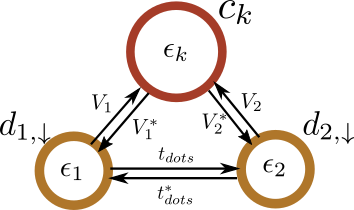
\includegraphics[scale=0.7]{IMAGES/Graphs/DQD.png}
    \caption{ Graph $\GDQD$  \protect\Source{By the author.}}
    \label{fig:graphDQD}
\end{figure}


Now, the Green functions $\Green{d_{1},d_{1}^{\dagger}}$ will always have the form $\frac{1}{\omega-E} $ where $E$ is an energy. This form is also observed in \ref{eq:solGreen}.  Looking at equation \ref{eq:green1},  observe that if $\Green{d_{2},d_{1}^{\dagger}}$ and $\sum_{\mathbf{k}}\Green{c_{\mathbf{k}},d_{1}^{\dagger}}$ are multiples of $\Green{d_{1},d_{1}^{\dagger}}$ (i.e $\Green{d_{2},d_{1}^{\dagger}}=\eta_{2}\Green{d_{1},d_{1}^{\dagger}},\Green{c_{\mathbf{k}},d_{1}^{\dagger}}=\eta_{\boldsymbol{k}}\Green{d_{1},d_{1}^{\dagger}})$ , the result for $\Green{d_{1},d_{1}^{\dagger}}$ will be 
\begin{equation}
    \Green{d_{1},d_{1}^{\dagger}}=\frac{1}{\omega-\epsilon_{1}-\sum_{\boldsymbol{k}}V_{1}^{*}\eta_{\boldsymbol{k}}+t_{dots}\eta_{2}}.
\end{equation}

Hence to obtain $\Green{d_{1},d_{1}^{\dagger}}$ we need to find $\eta_{\boldsymbol{k}}$ and $\eta_{2}$. Now note from equation \eqref{eq:green2} that $\left(\omega-\epsilon_{\boldsymbol{k}}\right)\eta_{\boldsymbol{k}}=V_{1}+V_{2}\eta_{2}$

\begin{equation}
\Green{d_{1},d_{1}^{\dagger}}=\frac{1}{\omega-\epsilon_{1}-\sum_{\boldsymbol{k}}\frac{V_{1}^{*}V_{1}}{\omega-\epsilon_{\boldsymbol{k}}}+V_{1}^{*}V_{2}t_{dots}\eta_{2}\eta_{2}}    
\end{equation}


Now, probably at this point you might already know what is happening here. Basically the energy $E$ represents the sum of all possible transitions in the graph that start and finish at $d_{1}$ . The first term is $\epsilon_{1}$, which is the energy of dot $1$. The next term is $\frac{V_{1}^{*}V_{1}}{\omega-\epsilon_{\boldsymbol{k}}}$ which represents the transition $d_{1}\rightarrow c_{k}\rightarrow d_{1}$. Note that $\frac{V_{1}^{*}V_{1}}{\omega-\epsilon_{\boldsymbol{k}}}$ is basically the energy needed to go from $d_{1}$ to $c_{\boldsymbol{k}}$ and coming back divided by the energy "cost" of passing through $c_{\boldsymbol{k}}$ which is $\omega-\epsilon_{\boldsymbol{k}}$. The sum over $\textbf{k}$ can be ignored in this analysis. Now we can then explain why the last term in \eqref{eq:solGreen} is 
\begin{equation}
    \frac{\left(t_{dots}+\sum_{\mathbf{k}}\frac{V_{1}V_{2}^{*}}{\omega-\epsilon_{\mathbf{k}}}\right)\left(t_{dots}^{*}+\sum_{\mathbf{k}}\frac{V_{1}^{*}V_{2}}{\omega-\epsilon_{\mathbf{k}}}\right)}{\omega-\epsilon_{2}-\sum_{\mathbf{k}}\frac{\Gamma_{2}^{2}}{\omega-\epsilon_{\mathbf{k}}}}. \label{term}
\end{equation}

Firs note that $\left(t_{dots}+\sum_{\mathbf{k}}\frac{V_{1}V_{2}^{*}}{\omega-\epsilon_{\mathbf{k}}}\right)$ is the energy needed to go from $d_{1}$ to $d_{2}$. This could occur by passing through $c_{\boldsymbol{k}} \ \left(\sum_{\mathbf{k}}\frac{V_{1}V_{2}^{*}}{\omega-\epsilon_{\mathbf{k}}}\right)$ or going directly to $d_ 2$ $\left(t_{dots}\right)$. The term is multiplied by $\left(t_{dots}^{*}+\sum_{\mathbf{k}}\frac{V_{1}^{*}V_{2}}{\omega-\epsilon_{\mathbf{k}}}\right)$ which represents the opposed transition from $d_{2}$ to $d_{1}$.  Finally, we  divide this by the cost of passing through $d_{2}$ and $c_{\boldsymbol{k}}$. This is basically to multiply by the green function taking the point $d_{1}$ out of $\GDQD$ . This green function is


\begin{equation}
    \GreenG{d_2,d_2^\dagger}{\GDQD-d1}= \frac{1}{\omega-\epsilon_{2}-\sum_{\mathbf{k}}\frac{\Gamma_{2}^{2}}{\omega-\epsilon_{\mathbf{k}}}}.
\end{equation}
where $\GreenG{d_2,d_2^\dagger}{\GDQD-d_1}$ is the green function of $d_2,d_2^\dagger$ in the smaller graph $\GDQD-d_1$. 

The last equation not only explains the meaning of term \eqref{term} in equation \eqref{eq:solGreen}. It also gives us an iterative method to find the green function. To understand this, note that the solution in \eqref{eq:solGreen} can also be written as 

\begin{equation}
\left( \GreenG{d_{1},d_{1}^{\dagger}}{\GDQD} \right) ^{-1}= \omega - \epsilon_1- \sum_\textbf{k} E_{d_1c_k}^{\GDQD-d_2} \GreenG{c_\textbf{k}c^\dagger_\textbf{k}}{\GDQD-d_2-d_1}  - E_{d_1d_2}^{\GDQD} \GreenG{d_2,d_2^\dagger}{\GDQD-d_1} . \label{eq:solGreen}
\end{equation}
Where $E_{d_1c_k}^{\GDQD-d_2} = \sum_{\boldsymbol{k}}\frac{V_{1}^{*}V_{1}}{\omega-\epsilon_{\boldsymbol{k}}} $  represents the accumulated energy of going from $d_1$ to $c_k$ and coming back. The upper-index $\GDQD-d_2$ represents that at this step second dot is ignored. Similarly $E_{d_1d_2}^{\GDQD}$ is the numerator of \eqref{term}. It represents the energy accumulated in at going from $d_1$ to $d_2$. Since this time no point is ignored, the upper-index remains as $\GDQD$. \\

Now the amazing thing about the last equation is that it decomposes the green function $\GreenG{d_{1},d_{1}^{\dagger}}{\GDQD}$  into green functions of smaller graphs. This gives an iterative process to compute green functions using induction in graphs .  Now, as you might see, the complexity of these green functions reduce strongly after a single point is removed out of the graph . This makes green function computation a pretty simple task using the graph method. 

\Jesus{I promise a real proof of this fact to be included in the abstract. The idea is using induction in graphs  \ref{sec:AbsGraphmethod}. }

\subsection{Density of states of the non-interacting Double Quantum Dot \label{sec:GreedDQD}}
The only missing 

% --------------------------------------------------
\section{The Numerical Renormalization Group\label{sec:The-Numerical-Renormaliztion} (NRG) }

 At low energies a renormalization group approach is necessary to deal with the effects of high correlations. This implies that the divergent resistivity in Kondo model will be renormalized to a finite quantity. 
 
 
\Jesus{I need to reference Kondo equations. Include advantages}

In the 1970's G.Wilson created a numerical method to solve the Anderson model . This method receives the name of Numerical Renormalization Group (NRG) \citep{bulla_numerical_2008,wilson_renormalization_1975,krishna-murthy_renormalization-group_1980}. It consists of three basic steps :
\begin{enumerate}
\item To perform a numerical discretization of the energy spectrum in logarithmic intervals. 
\item To map the discretized model onto a semi-infinity chain Hamiltonian. 
\item  To diagonalize iteratively the chain hamiltonian . 
\end{enumerate}

The final result will be the spectrum of the Hamiltonian. Other important properties of the material such as density of states, conductivity, specific heat, susceptibility can also be computed. On this project we are mainly interested in the Density of States (DOS). The method used to compute the DOS is the Density Matrix numerical renormalization Group (DM-NRG). A complete description of this algorithm will be given in the followin sections.  \\

For now, we proceed to describe how the NRG is applied to solve the Anderson model in a QD:\\

\subsubsection{Logarithmic Discretization:}

We start with an Anderson model hamiltonian such as the one 
in \prettyref{eq:Anderson} without magnetic field

\begin{equation}
H=\frac{U}{2}+\sum_{\sigma}\left[\left(\epsilon_{d}+\frac{U}{2}\right)d_{\sigma}^{\dagger}d_{\sigma}+\frac{U}{2}(d_{\sigma}^{\dagger}d_{\sigma}-1)^{2}+\sum_{\mathbf{k}}\ep_{\mathbf{k}}c_{\mathbf{k}\sigma}^{\dagger}c_{\mathbf{k}\sigma}+V_{\mathbf{k}}d_{\sigma}^{\dagger}c_{\mathbf{k}\sigma}+V_{\mathbf{k}}^{*}c_{\mathbf{k}\sigma}^{\dagger}d_{\sigma}\right].\label{HamWilson}
\end{equation}

At low-energies we can assume that QD couples only to s-wave states in the leads\citep{krishna-murthy_renormalization-group_1980}. This implies that that the Fermi surface is contained
in a single, isotropic conduction band extending inside some fixed cutoffs $-D$ and $D$. Thus, $\epsilon_{\mathbf{k}}$ only depends on $\left|\mathbf{k}\right|$. This makes possible to transform the sum over $\mathbf{k}$ in
equation \ref{HamWilson} into an integral over $\epsilon$ between
the energy cutoffs
\begin{eqnarray}
H & =\sum_{\sigma} & \Biggl[\left(\epsilon_{d}+\frac{U}{2}\right)d_{\sigma}^{\dagger}d_{\sigma}+\frac{U}{2}(d_{\sigma}^{\dagger}d_{\sigma}-1)^{2}+\int_{-D}^{D}\mbox{d}\epsilon\ \epsilon c_{\epsilon\sigma}^{\dagger}c_{\epsilon\sigma}\nonumber \\
 &  & \qquad\qquad\qquad\qquad\qquad\qquad+\int_{-D}^{D}\sqrt{\rho_{\sigma}(\epsilon)}\mbox{d}\epsilon\ V_{\epsilon}d_{\sigma}^{\dagger}c_{\mathbf{k}\sigma}+V_{\epsilon}^{*}c_{\epsilon\sigma}^{\dagger}d_{\sigma}\Biggr].\label{eq:hamEnergy}
\end{eqnarray}


Here $c_{\epsilon\sigma}^{\dagger}$ creates an electron with energy
$\epsilon$ and $\rho_{\sigma}(\epsilon)$ is the density of states
of the system per spin, which appears in the integral due to the change
of variable from $\mathbf{k}$ to $\epsilon\propto\left|\mathbf{k}\right|^{2}.$
Finally, we ignore the energy dependence of $\rho$ and $V_{d}$ and
we replace them by their values in the Fermi energy (This approximation
has no great relevance which is justified in \citep{krishna-murthy_renormalization-group_1980})
and we renormalize the energy band doing the replacements $k=\frac{\epsilon}{D}$
and $c_{k\sigma}:=\sqrt{D}c_{\epsilon\sigma}$ so that \prettyref{eq:hamEnergy}
becomes

\begin{eqnarray}
H & = & D\sum_{\sigma}\Biggl[\frac{1}{D}\left(\epsilon_{d}+\frac{U}{2}\right)d_{\sigma}^{\dagger}d_{\sigma}+\frac{U}{2D}(d_{\sigma}^{\dagger}d_{\sigma}-1)^{2}+\int_{-1}^{1}\mbox{d}k\ kc_{k\sigma}^{\dagger}c_{k\sigma}\nonumber \\
 &  & \qquad\qquad\qquad\qquad\qquad\qquad\qquad+\sqrt{\frac{\Gamma}{\pi D}}\int_{-1}^{1}\mbox{d}k\ d_{\sigma}^{\dagger}c_{k\sigma}+c_{k\sigma}^{\dagger}d_{\sigma}\label{eq:Norm-HamEnergy}\\
 & = & H_{d}+D\sum_{\sigma}\Biggl[\int_{-1}^{1}\mbox{d}k\ kc_{k\sigma}^{\dagger}c_{k\sigma}+\sqrt{\frac{\Gamma}{\pi D}}\int_{-1}^{1}\mbox{d}k\ d_{\sigma}^{\dagger}c_{k\sigma}+c_{k\sigma}^{\dagger}d_{\sigma}\Biggr],
\end{eqnarray}


\begin{figure}[h]
\centering
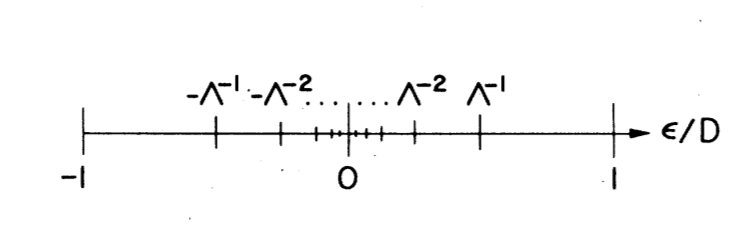
\includegraphics[scale=0.3]{IMAGES/Log-disc.png}\caption{\label{FigDiscretization} Taken from \citep{krishna-murthy_renormalization-group_1980}.
Energy interval discretization. \label{Energy-interval-discretization}}
\end{figure}


where $\Gamma=\pi\rho V^{2}$ is associated to the lever-width \citep[(3.5)]{sindel_numerical_2005}.
At this point we have our model dependent of three unit-less constants
$\frac{\epsilon_{d}}{D}\ ,\ \frac{U}{2D}$ and $\frac{\Gamma}{\pi D}$.
The logarithmic discretization starts by defining an scaling parameter
$\Lambda\geq1$ in diving the energy domain $[-1,1]$ into an array
of intervals of the form $\{[\pm\Lambda^{-(n+1)},\pm\Lambda^{n}]\}_{n\in\mathbb{N}}$,
as we can observe in \ref{FigDiscretization}. Note that the width
of these intervals is decreasing exponentially by 
\[
d_{n}=\Lambda^{-n}\left(1-\Lambda^{-1}\right).
\]


Then inside of these energy intervals we can define a set of orthonormal
Fourier series of the form
\begin{equation}
\phi_{np}^{\pm}(\epsilon)=\begin{cases}
\frac{1}{\sqrt{d_{n}}}e^{\pm i\omega_{n}p\epsilon} & \epsilon\in[\pm\Lambda^{-(n+1)},\pm\Lambda^{n}]\\
0 & \mbox{a.o.c },
\end{cases}\label{eq:orthonormal-Fourier}
\end{equation}


with $\omega_{n}:=\frac{2\pi}{d_{n}}$ so that $\phi_{np}^{\pm}\left(\pm\Lambda^{-(n+1)}\right)=\phi_{np}^{\pm}\left(\pm\Lambda^{-n)}\right).$
Then we can decompose the creation operators $c_{k}^{\dagger}$ into
their interval-Fourier contributions as 
\begin{equation}
c_{k\sigma}^{\dagger}=\sum_{np}\phi_{np}^{+}(k)c_{np\sigma}^{+\dagger}+\phi_{np}^{-}(k)c_{np\sigma}^{-\dagger}\label{eq:Fourier-interval decomposition}
\end{equation}


with the new creation operators defined as 
\[
c_{np\sigma}^{\pm\dagger}:=\left(c_{np\sigma}^{\pm}\right)^{\dagger}=\int_{-1}^{1}\mbox{d}\epsilon\ \left[\phi_{np}^{+}(\epsilon)\right]^{*}c_{\epsilon\sigma}^{\dagger}.
\]


This decomposition \prettyref{eq:Fourier-interval decomposition}
is a simple consequence of the orthonormality of the functions defined
in \prettyref{eq:orthonormal-Fourier}. In addition we can readily
proof that $c_{np\sigma}^{\pm\dagger}$-operators satisfy the anti-commutation
relations, so that they are rightful fermionic creation operators. 

We can now use \prettyref{eq:Fourier-interval decomposition} to replace
the $k$-dependent terms in hamiltonian \prettyref{eq:Norm-HamEnergy}.
Then we obtain

\begin{eqnarray}
\int_{-1}^{1}\mbox{d}k\ c_{k\sigma}^{\dagger}d_{\sigma} & = & \int_{-1}^{1}\mbox{d}k\ \left(\sum_{np}\phi_{np}^{+}(k)c_{np\sigma}^{+\dagger}+\phi_{np}^{-}(k)c_{np\sigma}^{-\dagger}\right)d_{\sigma}\nonumber \\
 & = & \left(\sum_{np}\left(\int_{-1}^{1}\mbox{d}k\ \phi_{np}^{+}(k)\right)c_{np\sigma}^{+\dagger}+\left(\int_{-1}^{1}\mbox{d}k\ \phi_{np}^{-}(k)\right)c_{np\sigma}^{-\dagger}\right)d_{\sigma}\nonumber \\
 & = & \left(\sum_{np}\left(\int_{\Lambda^{-(n+1)}}^{\Lambda^{-n}}\mbox{d}k\ \frac{e^{i\omega_{n}pk}}{\sqrt{d_{n}}}\right)c_{np\sigma}^{+\dagger}+\left(\int_{-\Lambda^{-n}}^{-\Lambda^{-(n+1)}}\mbox{d}k\ \frac{e^{-i\omega_{n}pk}}{\sqrt{d_{n}}}\right)c_{np\sigma}^{-\dagger}\right)d_{\sigma}\nonumber \\
 & = & \left(\sum_{np}\sqrt{d_{n}}\delta_{p}c_{np\sigma}^{+\dagger}+\sqrt{d_{n}}\delta_{p}c_{np\sigma}^{-\dagger}\right)d_{\sigma}\nonumber \\
 & = & \sqrt{1-\Lambda^{-1}}\sum_{n}\Lambda^{-\frac{n}{2}}\left(c_{np\sigma}^{+\dagger}+c_{np\sigma}^{-\dagger}\right)d_{\sigma}.\label{eq:firt-Integral}
\end{eqnarray}


And 

\begin{eqnarray}
\int_{-1}^{1}\mbox{d}k\ kc_{k\sigma}^{\dagger}c_{k\sigma} & = & \sum_{n,n',p,p'}\sum_{s,s'=\pm}\left(\int_{-1}^{1}k\mbox{d}k\ \phi_{np}^{s}(k)\left(\phi_{np}^{s'}(k)\right)^{*}\right)c_{np\sigma}^{s\dagger}c_{n'p'\sigma}^{s'}\nonumber \\
 & = & \sum_{n,n',p,p'}\sum_{s,s'=\pm}\left(\frac{\delta_{nn'}\delta_{ss'}}{d_{n}}\int_{\Lambda^{-(n+1)}}^{\Lambda^{-n}}k\mbox{d}k\ e^{is\omega_{n}k\left(p-p'\right)}\right)c_{np\sigma}^{s\dagger}c_{np'\sigma}^{s}\nonumber \\
 & = & \sum_{npp'}\sum_{s=\pm}\left(\frac{s}{2}\Lambda^{-2n}\left(1-\Lambda^{-2}\right)\delta_{pp'}+\frac{1-\delta_{pp'}}{is\omega_{n}\left(p-p'\right)}\left[ke^{is\omega_{n}k\left(p-p'\right)}\right]_{\Lambda^{-(n+1)}}^{\Lambda^{-n}}\right)\frac{c_{np\sigma}^{s\dagger}c_{np'\sigma}^{s'}}{d_{n}}\nonumber \\
 & = & \frac{1}{2}\left(1+\Lambda^{-1}\right)\sum_{np}\Lambda^{-n}\left(c_{np\sigma}^{+\dagger}c_{np\sigma}^{+}-c_{np\sigma}^{-\dagger}c_{np\sigma}^{-}\right)\nonumber \\
 &  & \ \ \ \ \ \ \!\ \ \ \ \!\ \ +\sum_{n}\sum_{p\neq p'}\frac{1-\Lambda^{-1}}{2i\pi\left(p'-p\right)}\left(c_{np\sigma}^{+\dagger}c_{np'\sigma}^{+}-c_{np'\sigma}^{-\dagger}c_{np\sigma}^{-}\right)e^{\frac{2i\pi\left(p-p'\right)}{1-\Lambda^{-1}}}.\label{eq:second-integral}
\end{eqnarray}


Thus, if we replace \prettyref{eq:firt-Integral} and \prettyref{eq:second-integral}
into \prettyref{eq:Norm-HamEnergy} we will obtain a logarithmic discretization
of the hamiltonian. The next part will we to map this discretization
to an iterative process that is worth for a numerical computations. 

\subsubsection{Mapping the Anderson model to a Chain-Hamiltonian}

\begin{figure}[h]
\centering
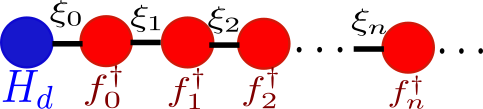
\includegraphics[scale=0.5]{IMAGES/NRGchain.png}\caption{\label{FigNRG-chain} Chain-Hamiltonian describing the Anderson model.
The chain starts at the initial dot hamiltonian $H_{d}$. The $f_{m}^{\dagger}$'s
are the creation operators at the $n^{\mbox{th}}$-site of the chain.
The $\xi_{n}$'s describe the magnitude of the interaction between
consecutive sites. }
\end{figure}


We are looking for a model just like the one we have in \ref{FigNRG-chain}.
This is because a Chain-Hamiltonian will give an iterative approximation
of the Anderson model with an increasing (but still controllable)
number of degrees of freedom. This will provide the rightful structure
for a numerical diagonalization of the hamiltonian. \\

To do this, observe from equations \prettyref{eq:firt-Integral},\prettyref{eq:second-integral}
that the QD ($d_{\sigma}$) couples directly only to the operators
with $p=0$$\left(c_{n0\sigma}^{\pm\dagger}\right)$. The $p\neq0$
terms will appear in the hamiltonian only because they are coupled
to $c_{np\sigma}^{+\dagger}$ in Equation \prettyref{eq:second-integral}.
Thus, as a first approximation we can neglect all terms in \prettyref{eq:second-integral}
with $p\neq0$. This leaves only the first part of \prettyref{eq:second-integral},
so that we can define $c_{n\sigma}^{\pm\dagger}:=c_{np\sigma}^{\pm\dagger}$
. Let 
\begin{equation}
f_{0\sigma}^{\dagger}=\sqrt{\frac{1-\Lambda^{-1}}{2}}\sum_{n}\Lambda^{-\frac{n}{2}}\left(c_{n\sigma}^{+\dagger}+c_{n\sigma}^{-\dagger}\right),\mbox{ so that }\sqrt{2}f_{0\sigma}^{\dagger}d_{\sigma}=\int_{-1}^{1}\mbox{d}k\ c_{k\sigma}^{\dagger}d_{\sigma}.\label{eq:f_0}
\end{equation}


Note $\left\{ f_{0\sigma}^{\dagger},f_{0\sigma}\right\} =\frac{1-\Lambda^{-1}}{2}\sum_{n}2\Lambda^{-n}=1$.
Replacing this in \prettyref{eq:Norm-HamEnergy}we get 
\[
H=H_{d}+D\sum_{\sigma}\Biggl[\sqrt{\frac{2\Gamma}{\pi D}}\left(d_{\sigma}^{\dagger}f_{0\sigma}+f_{0\sigma}^{\dagger}d_{\sigma}\right)+\frac{1}{2}\left(1+\Lambda^{-1}\right)\sum_{n}\Lambda^{-n}\left(c_{n\sigma}^{+\dagger}c_{n\sigma}^{+}-c_{n\sigma}^{-\dagger}c_{n\sigma}^{-}\right)\Biggr].
\]


$f_{0}^{\dagger}$will represent the first site of the chain-hamiltonian
in \ref{FigNRG-chain} since no other term is coupled to the dot hamiltonian.
We also have the coupling term $\xi_{0}=\sqrt{\frac{2\Gamma}{\pi D}}$.
It is possible to obtain the following $f_{m}^{\dagger}$-operators
by supposing a solution of the form 
\begin{equation}
f_{m\sigma}^{\dagger}=\sum_{n}a_{mn}^{+}c_{n\sigma}^{+\dagger}+a_{mn}^{-}c_{n\sigma}^{-\dagger}=\sum_{n}\sum_{s=\pm}a_{mn}^{s}c_{n\sigma}^{s\dagger},\label{eq:chain elements}
\end{equation}
 such that they satisfy the anti-commutation relations 
\[
\left\{ f_{m\sigma}^{\dagger},f_{m\sigma}\right\} =\delta_{mm'}\delta_{\sigma\sigma'}\ ,\ \left\{ f_{m\sigma}^{\dagger},f_{m\sigma}^{\dagger}\right\} =\left\{ f_{m\sigma}^{\dagger},f_{m\sigma}^{\dagger}\right\} =0
\]
and 
\begin{equation}
\frac{1}{2}\left(1+\Lambda^{-1}\right)\sum_{n}\Lambda^{-n}\left(c_{n\sigma}^{+\dagger}c_{n\sigma}^{+}-c_{n\sigma}^{-\dagger}c_{n\sigma}^{-}\right)=\sum_{m=0}^{\infty}\Lambda^{\frac{-m}{2}}\xi_{m}\left(f_{m\sigma}^{\dagger}f_{m+1,\sigma}+f_{m+1\sigma}^{\dagger}f_{m\sigma}\right).\label{eq:final equation}
\end{equation}


It is possible to find a solution for this system using the formula of
the right part of equation \ref{eq:final equation}. Since the relation
is only given between consecutive terms $m,m+1$ and we already have
the coefficients for $m=0$ $\left(a_{0n}^{s}=\sqrt{\frac{1-\Lambda^{-1}}{2}}\Lambda^{-\frac{n}{2}}\right).$
Then it is possible to determine the upper coefficients in a recursive way starting
from $m=0$. Supposing we can obtain the $m^{\mbox{th}}$-coefficients
$(a_{mn}^{s})$ and then finding iteratively the coefficients of $m+1\ (a_{mn}^{s})$
using the relation given by equation \prettyref{eq:final equation}.
This provides a numerical way for obtaining the $f_{m\sigma}^{\dagger}$
operators. In fact in our case, where we actually did important assumptions,
the problem can be solved analytically obtaining that the final hamiltonian
is given by 

\begin{equation}
H=H_{d}+D\sum_{\sigma}\Biggl[\sqrt{\frac{2\Gamma}{\pi D}}\left(d_{\sigma}^{\dagger}f_{0\sigma}+f_{0\sigma}^{\dagger}d_{\sigma}\right)+\frac{1}{2}\left(1+\Lambda^{-1}\right)\sum_{n=0}^{\infty}\Lambda^{\frac{-n}{2}}\xi_{n}\left(f_{n\sigma}^{\dagger}f_{n+1,\sigma}+f_{n+1\sigma}^{\dagger}f_{n\sigma}\right)\Biggr].\label{eq:chain-Hamiltonian}
\end{equation}


with 
\[
\xi_{n}=\frac{1-\Lambda^{-n-1}}{\left(1-\Lambda^{-2n-1}\right)^{\frac{1}{2}}\left(1-\Lambda^{-2n-3}\right)^{\frac{1}{2}}}.
\]


The formal recursive-solution of this problem can be found in \citep{bulla_numerical_2008}
. Note that equation \prettyref{eq:chain-Hamiltonian} describes the
chain hamiltonian model that we where looking for in \ref{FigNRG-chain}.
Note that in the limit when $n\longrightarrow\infty$ 

\[
\Lambda^{\frac{-n}{2}}\xi_{n}\longrightarrow\frac{\Lambda^{\frac{-n}{2}}\left(1-\Lambda^{-n}\right)}{1-\Lambda^{-2n}}\sim\frac{\Lambda^{\frac{-n}{2}}}{1+\Lambda^{-n}},
\]


which implies an exponential decaying of the hopping term in the chain. 

\subsubsection{Iterative Diagonalization in a Single QD process}

Now that we have an iterative representation of the Anderson Model
Hamiltonian \prettyref{eq:chain-Hamiltonian}, lets take a look to
how the NRG code would work for a QD. We start with the dot hamiltonian.
(Since the $D$ term is always present as a normalizing factor, we
are going to avoid this term in future computations and suppose that
we are working with unit-less variables $\epsilon_{d},\ U$ and $\Gamma':=\sqrt{\frac{2\Gamma}{\pi D}}$
).
\begin{equation}
H_{d}=\frac{1}{D}\left(\epsilon_{d}+\frac{U}{2}\right)d_{\sigma}^{\dagger}d_{\sigma}+\frac{U}{2D}(d_{\sigma}^{\dagger}d_{\sigma}-1)^{2}.\label{eq:DotHam}
\end{equation}


Now observe that hamiltonian \ref{eq:DotHam} already has a
diagonal form in the base $\left\{ \vert\uparrow\!\downarrow\rangle,\vert\uparrow\rangle,\vert\downarrow\rangle,\vert0\rangle\right\} $
\[
H_{d}=\frac{1}{D}\left[\begin{array}{cccc}
2\epsilon_{d}+\frac{3U}{2} & 0 & 0 & 0\\
0 & \epsilon_{d}+\frac{U}{2} & 0 & 0\\
0 & 0 & \epsilon_{d}+\frac{U}{2} & 0\\
0 & 0 & 0 & \frac{U}{2}
\end{array}\right].
\]


Lets define $H_{-1}=\Lambda^{\frac{-1}{2}}H_{d}.$ Adding the first
chain interaction to $H_{d}$ we obtain a new hamiltonian of the form 

\begin{equation}
H_{0}=\Lambda^{\frac{1}{2}}H_{-1}+\Gamma'\left(d_{\sigma}^{\dagger}f_{0\sigma}+f_{0\sigma}^{\dagger}d_{\sigma}\right).\label{eq:H0fromH-1}
\end{equation}


The Hilbert space for this hamiltonian has to be extended to include
the $4$ degrees of freedom of the $f_{0\sigma}^{\dagger}$ particles
which are also given by $\left\{ \vert\uparrow\!\downarrow\rangle,\vert\uparrow\rangle,\vert\downarrow\rangle,\vert0\rangle\right\} $.
Therefore the total Hilbert space for $H_{0}$ is given by a base
of the form 
\[
\vert s_{1}\rangle\vert s_{2}\rangle:=\vert s_{1}\rangle\otimes\vert s_{2}\rangle\mbox{ with }\vert s_{1,2}\rangle\in\left\{ \vert\uparrow\!\downarrow\rangle,\vert\uparrow\rangle,\vert\downarrow\rangle,\vert0\rangle\right\} .
\]


This gives an space of dimension $4\times4=16.$ Now before adventuring
to write the hamiltonian for $H_{0}$ as a $16\times16$-matrix note
that $H_{0}$ preserves particle number $N$ and the total spin $S$.
 Therefore we can use  $N$ and $S$ as quantum numbers and generate the Hamiltonian $H_{0}$ in blocks.
We will observe that the terms in the diagonal will correspond to
the eigenvalues of $H_{-1}$ for the first space. The non-diagonal
terms are the result of the hopping interactions with the first site. 

\begin{multicols}{2}

$H_{N=0,S=0}:$
\[
\begin{array}{c}
\vert0\rangle\vert0\rangle\rightarrow\end{array}\begin{array}{c}
\left[\frac{U}{2}\right]\end{array}
\]


$H_{N=4,S=0}:$
\[
\begin{array}{c}
\vert\uparrow\!\downarrow\rangle\vert\uparrow\!\downarrow\rangle\rightarrow\end{array}\begin{array}{c}
\left[2\epsilon_{d}+\frac{3U}{2}\right]\end{array}
\]


\end{multicols}

\begin{multicols}{2}

$H_{N=1,S=\frac{1}{2}}:$
\[
\begin{array}{c}
\vert\uparrow\rangle\vert0\rangle\rightarrow\\
\vert0\rangle\vert\uparrow\rangle\rightarrow
\end{array}\left[\begin{array}{cc}
\epsilon_{d}+\frac{U}{2} & \Gamma'\\
\Gamma' & \frac{U}{2}
\end{array}\right]
\]


$H_{N=1,S=\frac{-1}{2}}:$
\[
\begin{array}{c}
\vert\uparrow\rangle\vert0\rangle\rightarrow\\
\vert0\rangle\vert\uparrow\rangle\rightarrow
\end{array}\left[\begin{array}{cc}
\epsilon_{d}+\frac{U}{2} & \Gamma'\\
\Gamma' & \frac{U}{2}
\end{array}\right]
\]


\end{multicols}

\begin{multicols}{2}

$H_{N=2,S=-1}:$
\[
\begin{array}{c}
\vert\downarrow\rangle\vert\downarrow\rangle\rightarrow\end{array}\begin{array}{c}
\left[\epsilon_{d}+\frac{U}{2}\right]\end{array}
\]


$H_{N=2,S=1}:$
\[
\begin{array}{c}
\vert\uparrow\rangle\vert\uparrow\rangle\rightarrow\end{array}\begin{array}{c}
\left[\epsilon_{d}+\frac{U}{2}\right]\end{array}
\]


\end{multicols}

$H_{N=2,S=0}:$
\[
\begin{array}{c}
\vert\uparrow\!\downarrow\rangle\vert0\rangle\rightarrow\\
\vert\uparrow\rangle\vert\downarrow\rangle\rightarrow\\
\vert\downarrow\rangle\vert\uparrow\rangle\rightarrow\\
\vert0\rangle\vert\uparrow\!\downarrow\rangle\rightarrow
\end{array}\left[\begin{array}{cccc}
2\epsilon_{d}+\frac{3U}{2} & \Gamma & -\Gamma & 0\\
\Gamma & \epsilon_{d}+\frac{U}{2} & 0 & \Gamma\\
-\Gamma & 0 & \epsilon_{d}+\frac{U}{2} & -\Gamma\\
0 & \Gamma & -\Gamma & \frac{U}{2}
\end{array}\right]
\]


\begin{multicols}{2}

$H_{N=3,S=\frac{1}{2}}:$
\[
\begin{array}{c}
\vert\uparrow\!\downarrow\rangle\vert\uparrow\rangle\rightarrow\\
\vert\uparrow\rangle\vert\uparrow\!\downarrow\rangle\rightarrow
\end{array}\left[\begin{array}{cc}
\epsilon_{d}+\frac{U}{2} & -\Gamma'\\
-\Gamma' & \frac{U}{2}
\end{array}\right]
\]


$H_{N=3,S=\frac{-1}{2}}:$
\[
\begin{array}{c}
\vert\uparrow\!\downarrow\rangle\vert\downarrow\rangle\rightarrow\\
\vert\downarrow\rangle\vert\uparrow\!\downarrow\rangle\rightarrow
\end{array}\left[\begin{array}{cc}
\epsilon_{d}+\frac{U}{2} & -\Gamma'\\
-\Gamma' & \frac{U}{2}
\end{array}\right]
\]


\end{multicols}

Finally, we proceed to diagonalize $H_{0}$ by blocks $H_{N,S}$.
The resulting eigenvectors will be characterized by both quantum numbers
so that we can write them in the form $\vert N,S,i\rangle$ with $i$
takes as many values as the degeneracy of its block. For higher values of $N$,
the general formula for equation \prettyref{eq:H0fromH-1} looks as 
\begin{equation}
H_{N+1}=\Lambda^{\frac{1}{2}}\left[H_{N}+\frac{1}{2}\left(1+\Lambda^{-1}\right)\xi_{N}\left(f_{N\sigma}^{\dagger}f_{N+1,\sigma}+f_{N+1\sigma}^{\dagger}f_{N\sigma}\right)\right].\label{eq:NRG-Iteration Hamiltonians}
\end{equation}


We now proceed by induction supossing that for each $N$ the Hamiltonian $H_{N}$ is already diagonalized and the eigenvectors are organized in states with labels $\vert N,S,i\rangle.$ The next step will be to add the $4$-Hilbert space corresponding to $f_{N+1,\sigma}$ organized the eigenvectors according to the quantum numbers $\vert N',S',i\rangle$ and proceed to diagonalize by blocks the new Hamiltonian. Apart of it, the code must have a cutoff to the number of states. \\

This NRG code was previously implemented in C++ language by the advisor of this thesis. In \ref{Fig-Dot-Spectrum} we observe the evolution of the spectrum of the Hamiltonian according to the number of iterations of the code. As we can appreciate, this evolution converges for even and odd number around $N=30$. \\

\begin{figure}[h]
\subfloat[$N$ run only through even values]{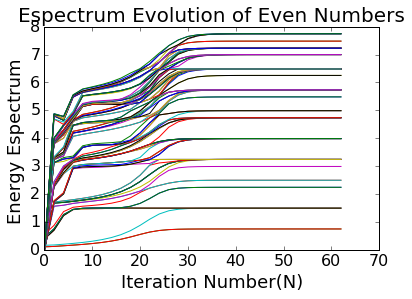
\includegraphics[scale=0.5]{IMAGES/even.png}}\subfloat[$N$ run only through odd values]{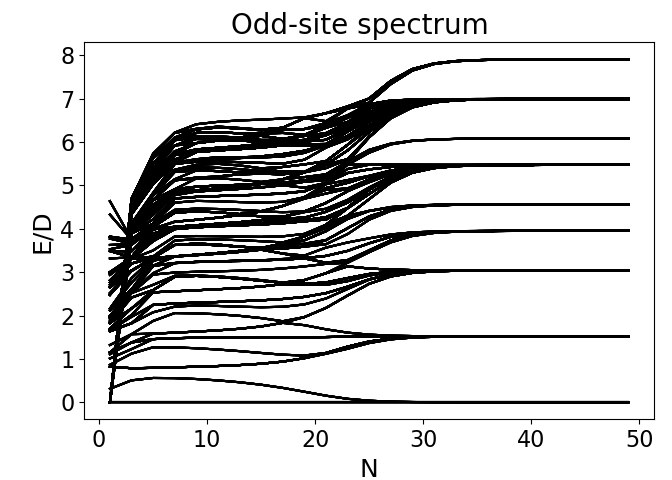
\includegraphics[scale=0.5]{IMAGES/odd.png}}\caption{\label{Fig-Dot-Spectrum} Evolution of the QD-spectrum vs number of
iterations of the code for $U=0.5,\ e_{d}=-0.25,\ \Gamma=2.82\times10^{-2}.$ }
\end{figure}
\section{Density Matrix Renormalization Group (DM-NRG)}

\section{NRG of the Kondo Effect}
